\documentclass[tikz,border=5pt]{standalone}
\usepackage{pgfplots}
\pgfplotsset{compat=1.12}
\usepgfplotslibrary{fillbetween}
\usepgfplotslibrary{polar}
\begin{document}
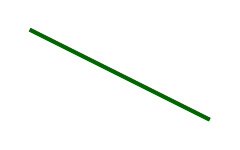
\begin{tikzpicture}[scale=0.5]
   \begin{polaraxis}[hide axis]
   \begin{scope}[]
        \addplot+[mark=none,domain=0:720,samples=100,line width=1mm,black!60!green,name path=B] {2 / (2*sin(x) + cos(x) )};
    \addplot+ [mark=none,domain=720-180:0,samples=100,line width=1mm,blue,name path=A] {0};   
    \tikzfillbetween[of=A and B,on layer=,split,every even segment/.style={fill=none,draw=red!80!black}]{red!80!black}  
  \end{scope}
    \end{polaraxis}
  \end{tikzpicture}
\end{document}